
\section{Safety} \label{Safety}

This section is going to look at regulations and legislation. Furthermore, continuing this section, a risk analysis is going to evaluate different situations.

\subsection{Regulations \& Legislation} \label{Regulationslegislations}
The Danish Traffic Laws has to be taken into consideration when developing an autonomous car.\cite{TrafficLaws} The car still has to follow the the laws when driving around, otherwise it would not be reliable. These are laws such as stopping at a red light and driving in the correct lane, as well as following all the road signs such as not going above the speed limit or stop at a duty to yield sign. With the right algorithms a car with the necessary sensors would be able to detect various obstacles, lights and signs. This will make it possible for the car to follow the law. As of right now the laws in Denmark prohibits autonomous cars from entering the road. It is not because the technology is not good enough, but rather because there is uncertainty as to where the liability lies if an accident happens.\cite{Illigle}

\noindent There are other places in the world where the autonomy in cars is allowed. As mentioned in \ref{Existing technologies} Starship technologies have had permission to deploy their robots in London , Washington and Hamburg, as well as the Waymo just recieved permission to test their vehicles on the road in California.\cite{DeliverySystem}

\subsection{ Environment and Obstacles } \label{Environmentobstacles}
In general, the traffic flow can be divided into two main categories; the urban road networks and the interurban, or rural, road network. As the road quality and the mix of traffic differ between the two networks, there is a need to look into these two networks.\cite{EUen}\\

\noindent Accident locations in urban areas are often scattered rather than on certain black spots as one sees in the rural network. 
Accidents that happen at these locations also differ. In the urban area, accidents often involve children, older people, pedestrians and cyclists.\cite{UCE}\\Which leads to the different obstacles that must be avoided in order to drive safely in both rural and an urban environment. 

\subsubsection{Obstacles}
One can categorise different obstacles in to multiple categories; Stationary objects, moving objects, wild life and people. It is clearly beneficial to be able to put obstacles into the relevant categories, in order for an avoiding system to be efficient. By correctly assessing different obstacles an avoidance system is able to differentiate the environment risk and how to handle in an emergency situation. 
\begin{table}[H]
    \centering
    \begin{tabular}{|@{\hspace{0.5cm}}c@{\hspace{0.5cm}}||@{\hspace{0.5cm}}c@{\hspace{0.5cm}}||@{\hspace{0.5cm}}c@{\hspace{0.5cm}}||@{\hspace{0.5cm}}c@{\hspace{0.5cm}}|}
    \hline
    \textbf{Stationary Objects} & \textbf{Moving Objects} & \textbf{Wildlife} & \textbf{Humans} \\ \hline
    Parked Cars                 & Cars                    & Dogs              & Children        \\
    Trees                       & Bicycles                &                   & Adults          \\
    Traffic signs                &                         &                   &                 \\ \hline
    \end{tabular}
    \caption{Examples of obstacles in every category of obstacles}
    \label{tab:my_label}
\end{table}

\subsection{Risk Assessment} \label{riskassessment}
In order to use an autonomous car for driving on the road, a risk assessment has to be completed. Therefore, this section is going to discuss the main risks of using autonomous cars. \\

\noindent  When a car is used for driving in the city the risk of surrounding people and other vehicles should be taken into consideration. The autonomous car should be able to detect people and cars around it and act depending on the situation. For instance, it should stop immediately if it detects a person or car in front. Furthermore, if there are any cars crashed on the road the autonomous car has to avoid them or just stop in front of the accident.\\

\noindent  Secondly, if the car is targeted in the car crash it is supposed to have safety features. For instance, seat belts and airbags to protect any passengers from a car crash.\\
Moreover, cars are supposed to have a braking system even though it is driving autonomously but it also has to allow a person to manually brake in order to stop in case of emergency. \\

\noindent  Another issue for the functionality of autonomous cars is their use in varying weather conditions. As such the car needs to be able  to detect the weather and road conditions to ensure the proper measures are taken if for example, the road is slippery or wet, what type of road it is and more. When the car is detecting the type of road and weather condition it should decide the suitable driving speed. Furthermore, if it is raining or snowing it has to clean windows of the car in order for the passenger to see the road. \\

\noindent  Moreover, animals on the road also have to be taken into consideration. The autonomous car has to detect big animals such as deer and small animals for example cats or dogs in order to keep passengers and animals safe. The main problem for detecting animals is that animals show up on the road unexpectedly. In addition to this, the autonomous car has to react within two seconds periode and it should act accordingly to the problem for example stop or if it is possible, avoid the animal. \\
%\todo[inline]{Need to add concrete information in risk assessment}

In conclusion, the autonomous car has to detect people and other cars on the road also animals and act accordingly to the situation. Furthermore, the car supposed to have safety features like brakes, seat belts and airbags for people in the car in as to lessen the possible injuries in a crash. Moreover, as detecting peoples and other cars it should also detect what weather is outside and set appropriate speed and controls. 


%https://www.futurecar.com/1262/Autonomous-Cars-are-Having-Trouble-With-Animals

%https://www.wired.com/story/trolley-problem-teach-self-driving-car-engineers/

%http://www.vejdirektoratet.dk/da/om-os/kampagner/holdafstand/sider/default.aspx

\section{Ethics}\label{Ethics}

\todo[inline]{Make a discussion}
\todo[inline]{Refer to any scientific papers done on the topic}
When programming a self driving car to avoid obstacles, it is important to classify what is an obstacle and what is not. If a small animal ran across the road, the car should try to avoid it, but if it turns out to be a plastic bag, it might have caused unnecessary turmoil in the traffic. If a person walks out in front of a car, and the driver swerves around to avoid the pedestrian, but this results in an other accident, the driver has now driven onto the sidewalk and into two other people. The driver of the car made a split second decision, whether to swerve or not. Had the driver not turned the wheel, they would have driven into the crossing pedestrian. A lot of factors play into the decisions the driver makes. Were they not aware of the people on the sidewalk? It could have been a loved one on the street. Maybe it was a child who ran in front of the car and the driver would rather spare a kid. All these questions are ethical, and answers vary a lot depending on where in the world you are and who you are as a person.\cite{Ethics}\\

\noindent The trolley problem refers to the morality involved in certain situations where human life is in danger, and if it truly is better to kill one than many. This problem is also relevant when designing the control system of an autonomous car, as the system would in some dire situations need to choose, weather to kill an individual or a group. \\
This problem has been discussed by philosophers for many years with no definitive answer. 

\noindent The trolley problem says what should self-driving cars do if it is in a situation where it should choose to kill one person or multiple. This question was analysed for a long time. But according to discussions and situations, the car has to have a system which supposed to detect this situation before it happens and stop immediately. \\

\noindent When the programmer has to program what to do in a given scenario, they have to evaluate the value of all possible "obstacles", be it trashcans, lampposts, animals or humans. If a scenario rises where the car cannot avoid a collision, what should the outcome be. For a human driver the decision is made in a split second, and possibly the driver had not gotten all the details of the situation. For a self driving car, it can be assumed all the details are know to the car. This of course depends on the quality and quantity of sensors and cameras, but this will be ignored. The car will have to compare the different outcomes and choose the action that results in the least damage. All of this goes back to the programmer of the car. They are the ones to classify and put a value on the individual based on what can be observed by the car. As mentioned before, this vary from country to country.\\

\noindent One might argue to save the younger over the elder, or save women over men. This is a discussion that can go on forever, without a definitive conclusion. A survey has been made that compares the moral choices of people from different parts of the world. $2,3$ million people were involved, and it gives a good picture on how diverse opinions can be.\\
\begin{figure}[H]
\centering
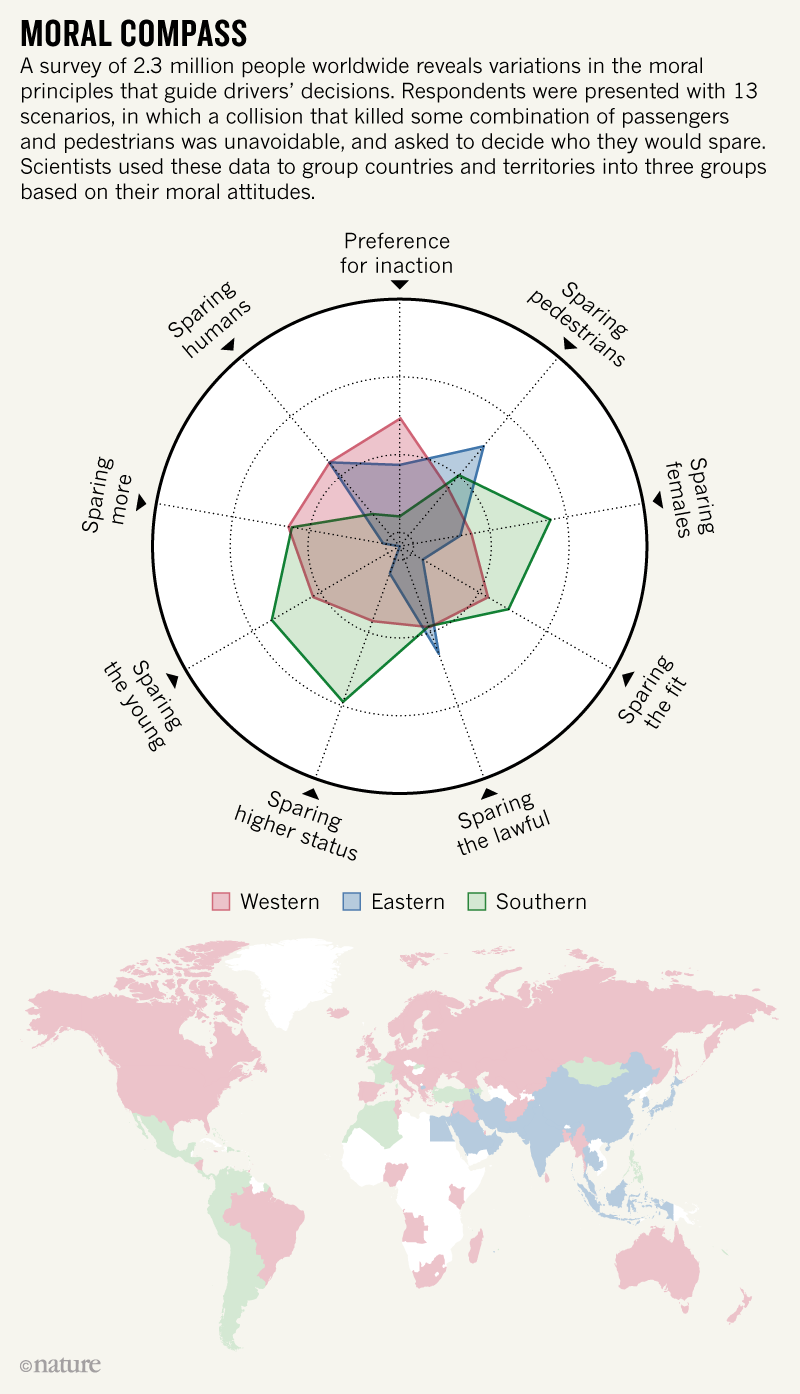
\includegraphics[width=\textwidth]{Figures/ConAnalysis/General/MoralCompass.png}
\caption Moral compass of different parts of the world{\cite{Ethics}}
\end{figure}

\\
\todo[inline]{Scale picture}
\noindent As seen from the picture above, a single programmer can not decide for the whole world, how the car should behave when facing such decisions.
\todo[inline]{Needs a conclusion how this will affect the project solution}
